\begin{figure*}[t]
\begin{center}
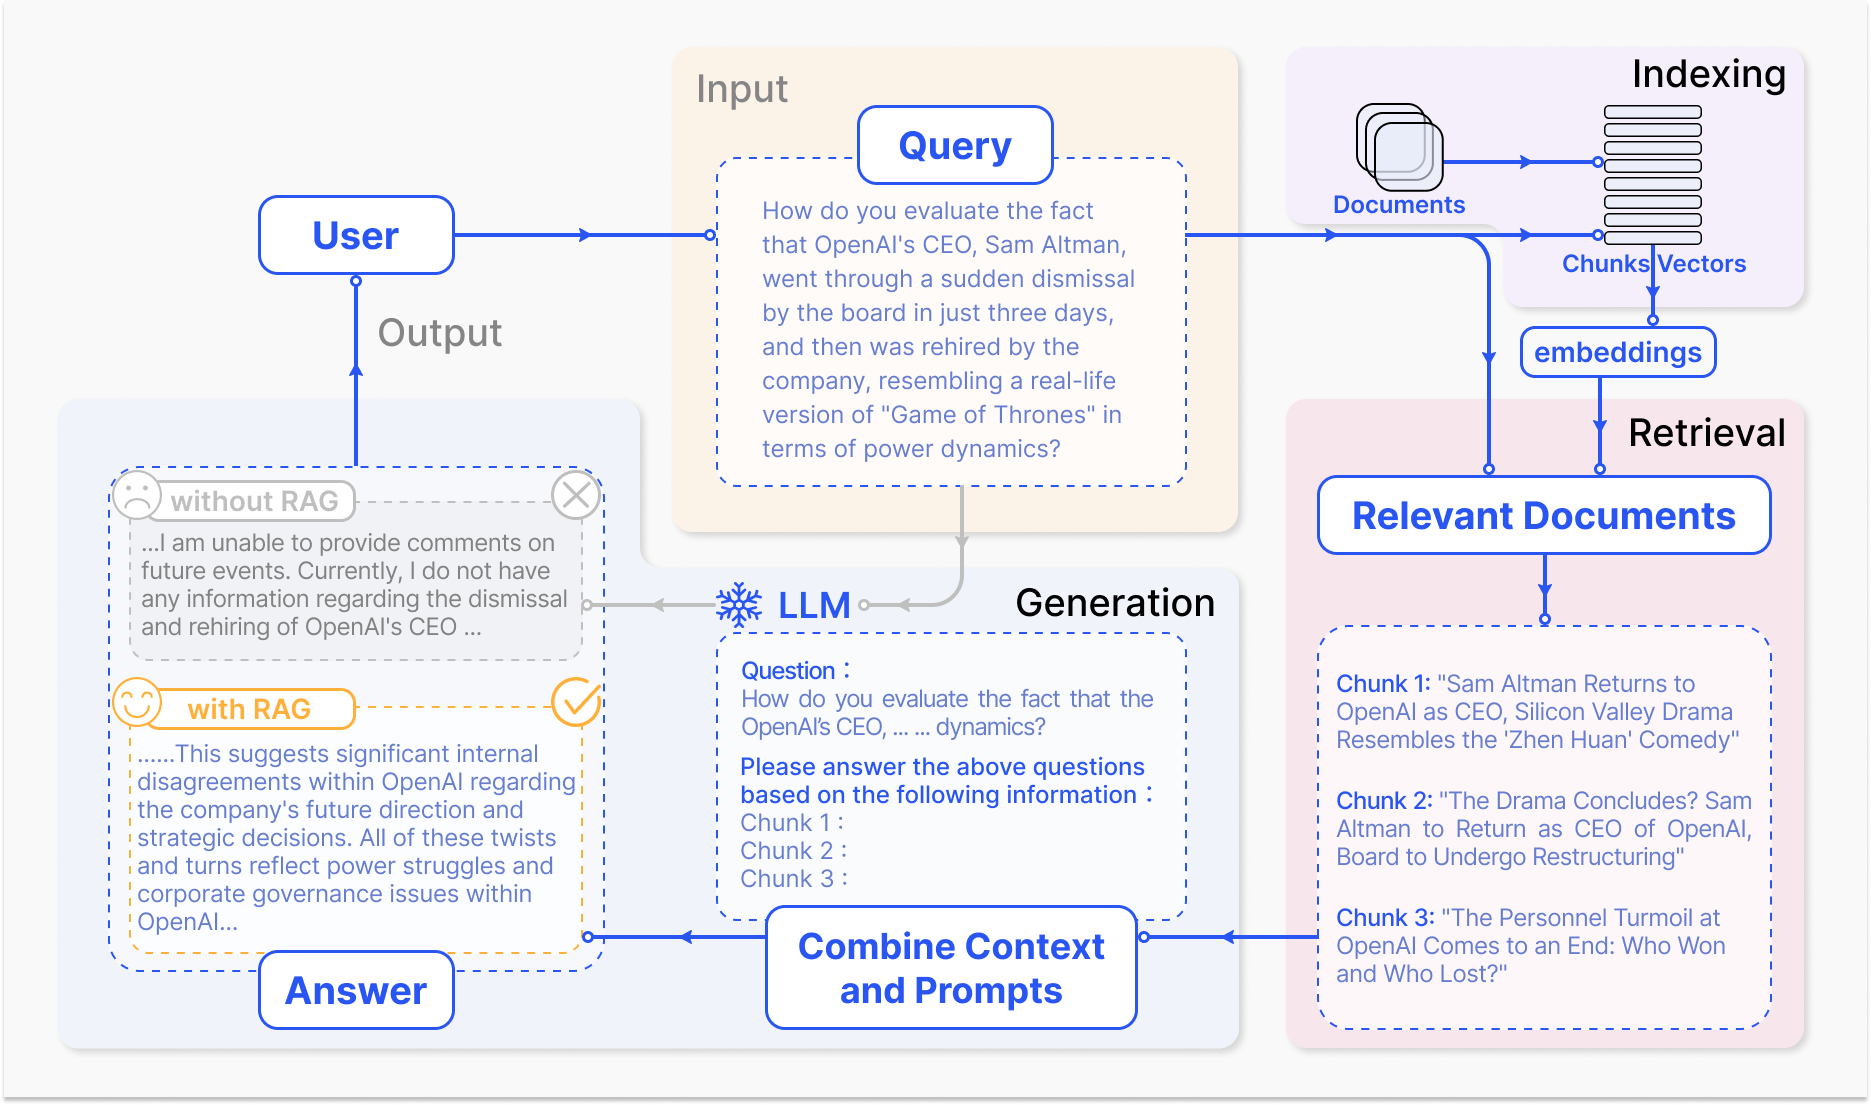
\includegraphics[width=0.9\textwidth]{images/RAG_case.png}
\end{center}
\caption{
Architecture of Retrieval-Augmented Generation (RAG)~\citep{gao2024retrievalaugmented}: factual knowledge is stored in a key-value memory where keys and values correspond to questions and answers, respectively;
during inference, the model retrieves information from the memory via similarity search and uses it to condition the generation process.
}
\label{fig:arch}
\end{figure*}

\section{Project Overview}

\subsection{Datasets}

The dataset utilized in this study is the \emph{nq\_open} validation dataset, hosted on HuggingFace (\url{https://huggingface.co/datasets/nq_open/viewer/nq_open/validation}). This validation dataset, introduced by~\citep{lee-etal-2019-latent}, comprises 3,610 question-answer pairs and serves as a benchmark for open-domain question answering, derived from \emph{NaturalQuestions}. The objective is to predict an English answer string for a given English question.

\subsection{Knowledge Source}

The \emph{PAQ} dataset~\citep{paq} serves as the knowledge source and is available on GitHub (\url{https://github.com/facebookresearch/PAQ?tab=readme-ov-file#paq-qa-pairs}). The QA pairs in PAQ were trained and retrieved from \emph{NaturalQuestions} and \emph{TriviaQA}, with the full version containing 64.9M QA pairs. For this project, We utilized \emph{PAQ-L1}, a lighter version of \emph{PAQ} with 14.1M QA pairs. Although \emph{PAQ-L1} has more than four times fewer data rows, it still maintains substantial coverage of \emph{NQ} (88.3\%) and \emph{TQA} (90.2\%) compared to the full \emph{PAQ} version, which covers \emph{NQ} (90.2\%) and \emph{TQA} (91.1\%)~\citep{paq}. Since the \emph{PAQ} data is derived from \emph{NaturalQuestions}, it encompasses the coverage of the \emph{nq\_open} dataset mentioned earlier and is thus a suitable candidate for a knowledge source in knowledge augmentation generation.

\begin{table}
\renewcommand\arraystretch{1.2} 
\setlength\tabcolsep{4pt}
\centering
\resizebox{\columnwidth}{!}{
    \begin{tabular}{ll}
    \toprule
    \multicolumn{2}{c}{\textbf{Natural Question (\emph{PAQ})}} \\ \midrule
    \textbf{Q}: where is conan meriadoc from? & \textbf{A}: \emph{british} \\ \midrule
    \multicolumn{2}{l}{\textbf{Retrieved Key-Values}} \\
    \textbf{Q}: who is conan meriadoc mentioned alongside in & \textbf{A}: cadwaladr \\ armes prydein? \\
    \textbf{Q}: who argued that conan meriadoc dates back to  & \textbf{A}: hubert guillotelr \\ the mid 12th century? \\
    \textbf{Q}: conan meriadoc was the roman name for whom? & \textbf{A}: magnus maximus \\
    \textbf{Q}: who is the compiler of conan meriadoc? & \textbf{A}: gurheden \\
    \textbf{Q}: what nationality was conan meriadoc? & \textbf{A}: \underline{\emph{british}} \\
    \bottomrule
    \end{tabular}
}
    \caption{Example question from \emph{PAQ} and its associated answer, along with the top-5 question-answer pairs retrieved from the vector store by similarity search.}
    \label{tab:paq_with_scores}
\end{table}

\subsection{Build Knowledge}

The process of building knowledge is crucial for knowledge retrieval and augmentation. The aim is to transform the raw \emph{PAQ-L1} data, which consists of question-answer text pairs, into key-value knowledge embeddings, using the question as the embedding key. The choice of the embedding model is also significant, as it impacts the precision of knowledge compression and retrieval, as well as the speed of embedding computation. After thorough research and considering both accuracy and efficiency, \emph{BAAI/bge-small-en}~\cite{bge_embedding} was chosen for its lower computational demand yet competitive performance. This model is based on the English language and has an embedding size of 384. Given that both the knowledge source and the evaluation dataset consist of brief questions and answers, an embedding size of 384 is deemed sufficient to encapsulate the relevant information.

Given the limited GPU computing power, a batch size of 500 for the embedding computation step has been determined. The embedded QA pairs are then stored in \emph{Pinecone} vector database and are integrated into a node retrieval object implemented by \emph{LlamaIndex} APIs. This retrieval object takes a question as the query text, computes its embedding using the same \emph{BAAI/bge-small-en} embedding model, and performs a vector similarity search in \emph{Pinecone}. The top-k embedded QA pairs are returned with their associated scores. \cref{tab:paq_with_scores} shows an example question and the top-5 retrieved answers from \emph{PAQ}.

Last, the question associated with the retrieved knowledge QA pairs with scores will be passed to LLMs for generation inference.

\subsection{Model Selection}

\emph{Flan-T5-base}: A variant of \emph{T5-base} with the same number of parameters (220 million) but has been fine-tuned on over 1,000 additional tasks~\citep{https://doi.org/10.48550/arxiv.2210.11416}. It outperforms \emph{T5-base} in many tasks, including question-answering. It has also been fine-tuned with instruction-based prompt texts, allowing it to utilize external knowledge to provide answers. Therefore, \emph{Flan-T5-base} has been selected as the baseline model. HuggingFace: \url{https://huggingface.co/google/flan-t5-base}

\vspace{0.3\baselineskip}

\noindent\emph{Flan-T5-large}: With an increased number of parameters (770 million), \emph{Flan-T5-large} retains all the features of \emph{Flan-T5-base} and represents a slight advancement over the baseline model.
HuggingFace: \url{https://huggingface.co/google/flan-t5-large} 

\vspace{0.3\baselineskip}

\noindent\emph{Llama-2-13B-chat-GGUF}: Similar to \emph{Llama-2-13B-chat-hf} except for its format, introduced by the \emph{llama.cpp} team. Llama 2 consists of a series of pretrained and fine-tuned generative text models developed by Meta~\citep{touvron2023llama}. In this study, we use the 13 billion parameter version of Llama 2, optimized for dialogue applications.
HuggingFace: \url{https://huggingface.co/TheBloke/Llama-2-13B-chat-GGUF} 

\vspace{0.3\baselineskip}

\noindent\emph{GPT-3.5-Turbo}: Provided by \emph{OpenAI}, \emph{GPT-3.5-Turbo} is considered state-of-the-art for many NLP tasks due to its highly adaptable prompt capability~\citep{brown2020language}. It is used as the most advanced LLM in this study. The current version, \emph{GPT-3.5-Turbo-0125}, features a 16,385-token context window and training data up to September 2021.
OpenAI: \url{https://platform.openai.com/docs/models/gpt-3-5-turbo}
